\documentclass[tikz,border=2pt]{standalone}
\usepackage{times}
\usepackage{amsmath,amssymb}
\usetikzlibrary{arrows.meta,calc,decorations.markings}
\definecolor{ink}{HTML}{0b0b0b}
\definecolor{sub}{HTML}{52514e}
\definecolor{axis}{HTML}{9a9994}
\definecolor{ours}{HTML}{0F4D92}
\definecolor{tint}{HTML}{E9EFF7}
\begin{document}
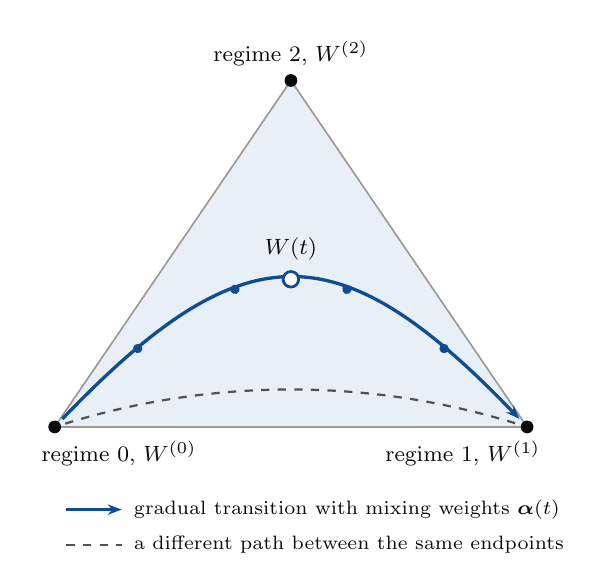
\begin{tikzpicture}[font=\footnotesize, text=ink, >={Stealth[length=5pt]}]
  \coordinate (A) at (0,0);
  \coordinate (B) at (6,0);
  \coordinate (C) at (3,4.4);
  \fill[tint] (A)--(B)--(C)--cycle;
  \draw[axis, line width=0.6pt] (A)--(B)--(C)--cycle;

  % another path between the same endpoints
  \draw[sub, dashed, line width=0.8pt, shorten <=4pt, shorten >=4pt]
        (A) .. controls (2.0,0.62) and (4.0,0.62) .. (B);

  % a gradual transition through the interior, with time steps marked
  \draw[ours, line width=1.2pt, ->, shorten <=4pt, shorten >=4pt,
        postaction={decorate, decoration={markings,
          mark=between positions 0.2 and 0.8 step 0.2 with {\fill[ours] (0,0) circle (1.7pt);}}}]
        (A) .. controls (2.4,2.5) and (3.6,2.5) .. (B);
  \coordinate (S) at (3,1.875);
  \fill[white] (S) circle (2.8pt);
  \draw[ours, line width=1pt] (S) circle (2.8pt);
  \node[anchor=south, inner sep=1pt] at ($(S)+(0,0.2)$) {$W(t)$};

  % atomic mechanisms at the vertices
  \foreach \p in {A,B,C}{ \fill[ink] (\p) circle (2.3pt); }
  \node[anchor=south, inner sep=5pt] at (C) {regime 2, $W^{(2)}$};
  \node[anchor=north west, inner sep=5pt] at ($(A)+(-0.35,0)$) {regime 0, $W^{(0)}$};
  \node[anchor=north east, inner sep=5pt] at ($(B)+(0.35,0)$) {regime 1, $W^{(1)}$};

  % legend below the simplex
  \draw[ours, line width=1.2pt, ->] (0.15,-1.05) -- (0.85,-1.05);
  \node[anchor=west, font=\scriptsize, inner sep=0pt] at (1.0,-1.05)
      {gradual transition with mixing weights $\boldsymbol{\alpha}(t)$};
  \draw[sub, dashed, line width=0.8pt] (0.15,-1.5) -- (0.85,-1.5);
  \node[anchor=west, font=\scriptsize, inner sep=0pt] at (1.0,-1.5)
      {a different path between the same endpoints};
\end{tikzpicture}
\end{document}
